We perform three sets of experiments to evaluate the model and the stochastic variational inference proposed. 
First, we use a toy problem to demonstrate the effectiveness of the proposed method in learning the model parameters.
Second, we assess the predictive accuracy of the model on two medium-sized datasets and compare with existing multiple output models.
In the final experiments, we evaluate the model on large-scale learning with multiple tasks.

\subsection{TOY PROBLEM}
In this toy problem we use two related outputs generated from the same latent function $sin(x)$ but are corrupted by independent noises: $y_1(x) = sin(x) + \epsilon$ and $y_2(x) = -sin(x) + \epsilon$, $\epsilon \sim \Normal(0,0.01)$.
Each output has missing values in one region of the input space.
% Say that this is from a single gpsvi
The predictive distributions of the model compared to that of independent gps are shown in \ref{fig5}.

\begin{figure*}
\centering
\begin{tabular}{cc}
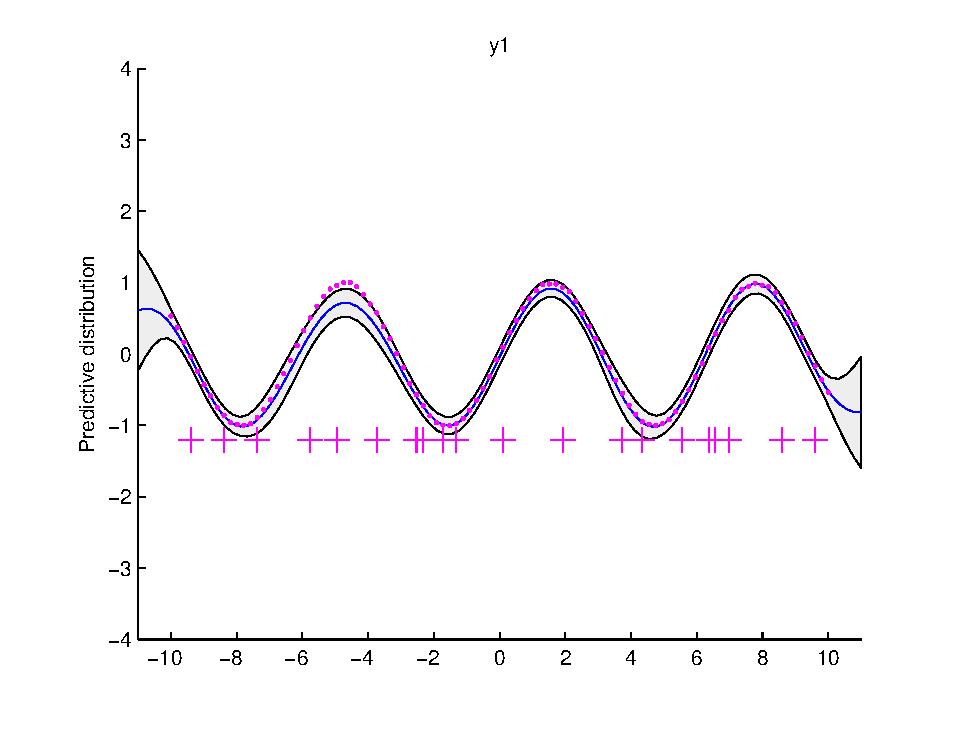
\includegraphics[scale=0.5]{figures/ssvi2-y1.eps} &
\includegraphics[scale=0.5]{figures/ssvi2-svi1.eps} \\
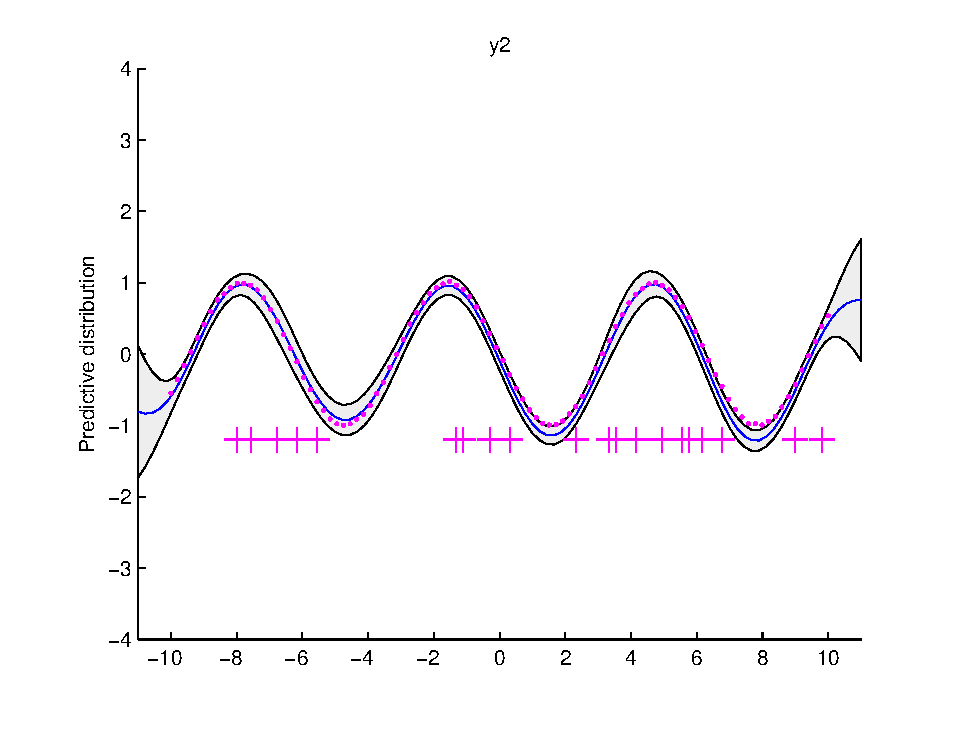
\includegraphics[scale=0.5]{figures/ssvi2-y2.eps} &
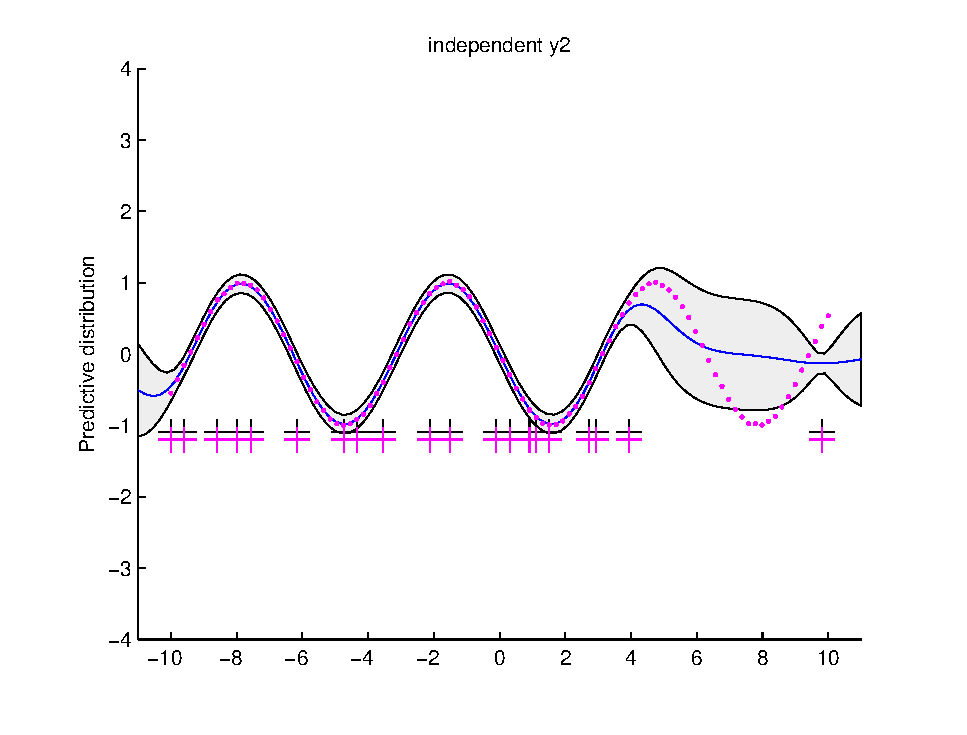
\includegraphics[scale=0.5]{figures/ssvi2-svi2.eps} \\
\end{tabular}
\label{fig5}
\caption{Predictive distributions of the multioutput gps (left column) and independent gps (right column) for the second toy experiment. The predictive distribution by $g(x)$ for $y_1(x)$ is shown in the bottom figure.}
\end{figure*}

\subsection{EVALUATION OF THE PREDICTIVE ACCURACY}
\subsubsection{Foregin Exchange Rate Prediction}
\subsubsection{Weather Data Prediction}

\subsection{LARGE-SCALE EXPERIMENTS}
\subsubsection{Robort Arms}
\subsubsection{Foreign Exchange Rate Prediction}
